\documentclass[xelatex,12pt]{beamer}
\usepackage{pgfpages}
\usepackage{fontspec}
\usepackage{xunicode}
\usepackage{polyglossia}
\PolyglossiaSetup{french}{indentfirst=false}
\usepackage[french=guillemets]{csquotes}
\usepackage{xpatch}
\usepackage{diagbox}

\setmainlanguage{french}
\xapptocmd\ttfamily{\XeTeXinterchartokenstate=0 }{}{}
\newcommand{\nospace}[1]{\texttt{#1}}

\usepackage{algorithm}
\usepackage[noend]{algpseudocode}
    \newcounter{lastenum}
    \newcommand{\mtpause}{\setcounter{lastenum}{\value{enumi}}}
    \newcommand{\mtresume}{\setcounter{enumi}{\value{lastenum}}}
\resetcounteronoverlays{lastenum}

\usepackage[backend=biber, style=chem-acs]{biblatex}
\addbibresource{Modele.bib} 
\setbeamertemplate{bibliography item}[triangle]

\setbeamertemplate{caption}[numbered]
 
\usepackage{multirow}% row fusion
\usepackage{array} % column fusion
\usepackage{xfrac} % small fractions
\usepackage{adjustbox}
\usepackage{listings}

\usepackage{color}
\definecolor{gray}{rgb}{0.4,0.4,0.4}
\definecolor{darkblue}{rgb}{0.0,0.0,0.6}
\definecolor{cyan}{rgb}{0.0,0.6,0.6}

\usetheme{Warsaw}

\setbeamertemplate{frametitle}{\nointerlineskip  
    \begin{beamercolorbox}[wd=\paperwidth,ht=2.75ex,dp=1.375ex]{frametitle}
        \hspace*{2ex}\insertframetitle \hfill {\small\insertframenumber/\inserttotalframenumber} \hspace*{1ex}%
    \end{beamercolorbox}}

\usecolortheme{wolverine}

\setbeameroption{hide notes} % Only slides
%\setbeameroption{show only notes} % Only notes
%\setbeameroption{show notes on second screen=right} % Both

 \titlegraphic{\vspace{-1cm}
      
\includegraphics[width=2.5cm]{images/logo_paris_8.png}\hspace*{4.75cm}~%
      \hfill
      
\includegraphics[width=2.5cm]{images/logo_junglebike.png}
}

 
\title{Système de Recommandation }
\subtitle{Apprentissage chez Junglebike}
\author[\textsc{Komlan DANTODJI}]{\textsc{Komlan Jean-Marie DANTODJI}}
\institute{\normalsize Université Paris 8, LIASD\\
Encadrante : Mme Rakia JAZIRI\\
Tutrice : Mme Alice Battarel
}
 
\beamertemplatenavigationsymbolsempty
\setbeamertemplate{blocks}[rounded][shadow=true]
\setbeamerfont{page number in head/foot}{size=\large}

\begin{document}
{ \setbeamertemplate{headline}{}
  \setbeamertemplate{footline}{}
  \begin{frame}
  \titlepage
  \end{frame}

\note{
}
}

  
\tableofcontents[sectionstyle=show/show, hidesubsections]
\note{
}  

\section{Introduction}
\subsection{Présentation de l'entreprise}
\begin{frame}{JungleBike}
\begin{itemize}
		\item Start Up de E-Commerce de B2B et B2C.
		\item Spécialisée dans le secteur du Vélo. 
		\item Mise en relation des clients avec les réparateurs.
\end{itemize}
\end{frame}

\section{Contexte} % pour l'exposé final, commenter
%\subsection{Contexte} % pour l'exposé final, décommenter

\begin{frame}{Contexte RH}
  \begin{itemize}
  \item Equipe Data 
  \item Formé de trois data scientistes
  \item Une responsable de l'équipe data
  \end{itemize}
\end{frame}

\begin{frame}{Contexte technique}
  \begin{itemize}
  \item Intégration de données
  \item Construction des algoritmes de catégorisation et d'extration de données
  \item Outils: DataIku, DBeaver
  \item Langages et librairies: Python, Scikit Learn, Keras, Tensorflow, PyTorch
  \end{itemize}
\end{frame}

\section{Problématique}

\subsection{Objectif}

\begin{frame}{Problème}
  \begin{itemize}
  \item Recommandation des produits basées sur le vote et avis des clients.
  \end{itemize}
\end{frame}

\subsection{Problematique des données}
\begin{frame}{Problematique des données}
\begin{itemize}
  \item L’information sur l’avis client.
  \item Biais de popularité: non diversité des produits recommandés
  \item Manque d’avis clients en comparaison au nombre d’article à recommander
  \item Données issues du scrapping des sites des fournisseurs.
  \end{itemize}
\end{frame}

\subsection{Données}
\begin{frame}{Données}
\begin{figure}[h]
\begin{center}
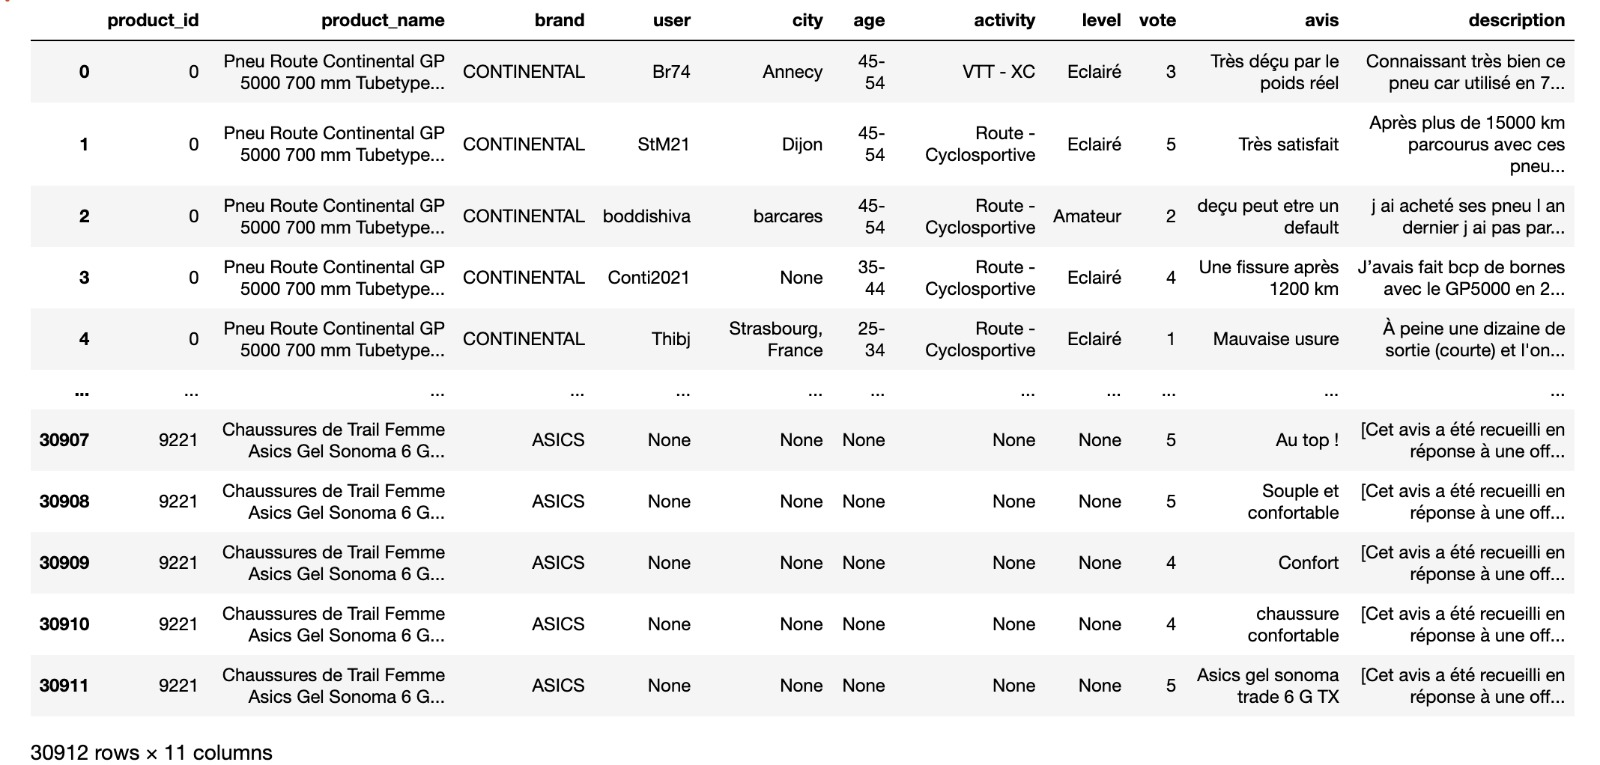
\includegraphics[width=11cm,height=5cm]{images/sample_data.jpeg}
\caption[Jeu de données issue du Scrapping des sites des fournisseurs]{Jeu de données issue du Scrapping des sites des fournisseurs}
\label{monlabel}
\end{center}
\end{figure}
\end{frame}


\subsection{Détail des colonnes}
\begin{frame}{Détail des colonnes}
\begin{figure}[h]
\begin{center}
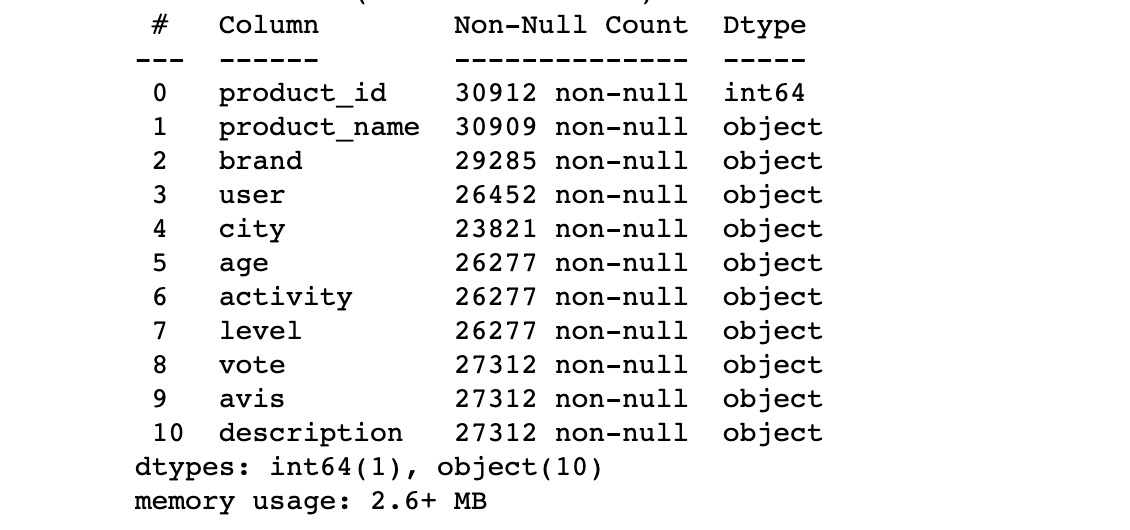
\includegraphics[width=12cm,height=4.8cm]{images/detail_columns.jpeg}
\caption[Détail des colonnes]{Détail des colonnes}
\label{monlabel}
\end{center}
\end{figure}
\end{frame}

\subsection{Méthodes de validation des modèles}
\begin{frame}{Validation de modèle}
MSE: Mean Squared Error:
$$
\mathrm{MSE}=\frac{1}{n} \sum_{i=1}^n\left(y_i-\hat{y}_i\right)^2
$$
RMSE: Root Mean Squared Error
$$
\mathrm{RMSE}=\sqrt{\frac{1}{n} \sum_{i=1}^n\left(y_i-\hat{y}_i\right)^2}
$$
MAE: Mean Absolute Error:
$$\mathrm{MAE}=\frac{1}{n} \sum_{j=1}^n\left|y_j-\hat{y}_j\right|
$$
\end{frame}



\section{État de l'art}
\subsection{Méthodes élémentaires}
\begin{frame}{Méthodes élémentaires}
\begin{itemize}
  \item Recommandation aléatoire
  \end{itemize}
\end{frame}

\subsection{Recommandation Objet (Content-Based filtering CB)}
\begin{frame}{Recommandation Objet}
\begin{itemize}
  \item Caracteristiques des produits
  \item Projection des produits dans un repere
  \end{itemize}
\end{frame}

\begin{frame}{Methode du Cosin Similarity}
\begin{figure}[h]
\begin{center}
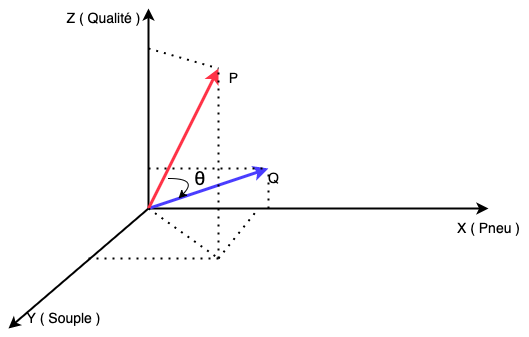
\includegraphics[width=8cm,height=4.5cm]{images/cosin_similarity.png}
\caption[Projection des produits]{Projection des produits}
\label{monlabel}
\end{center}
\end{figure}
\end{frame}


\subsection{Recommandation Sociale (Collaborative Filtering CF – Context Aware)}
\begin{frame}{La Matrice de Factorisation}
\begin{itemize}
  \item Décomposer la matrice de votes en deux
  \end{itemize}
  $$M = U x I$$
\end{frame}

\begin{frame}{Décomposition}
\begin{figure}[h]
\begin{center}
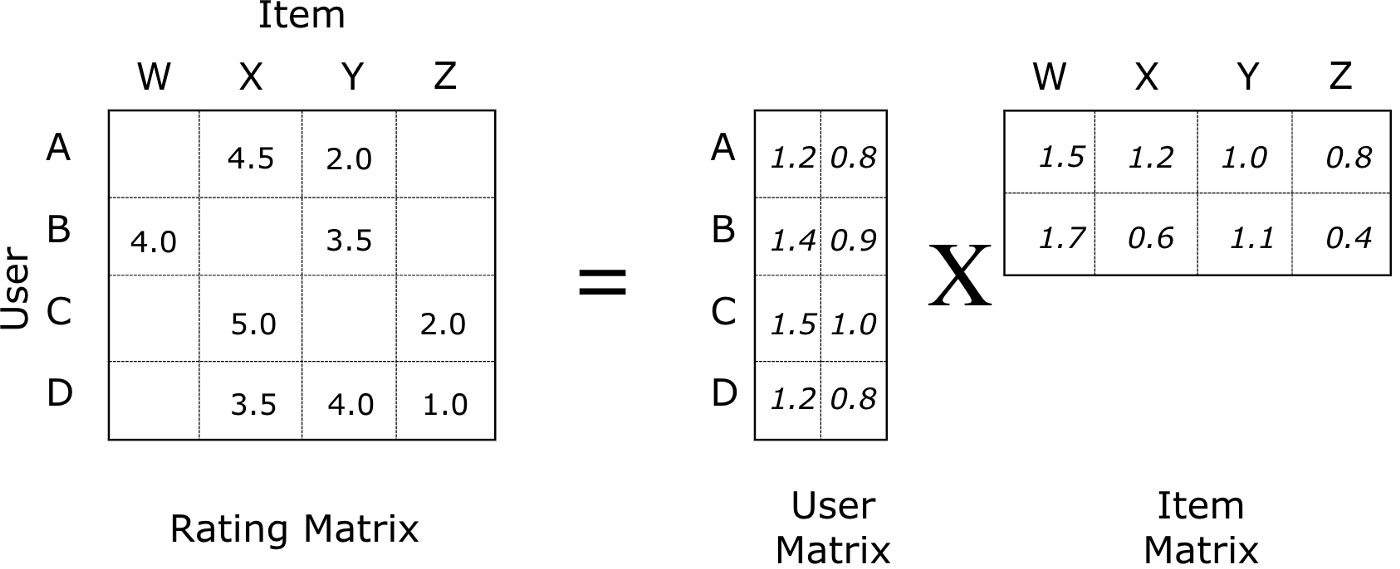
\includegraphics[width=11cm,height=4.8cm]{images/factorisation_matrix.png}
\caption[Décomposition de la matrice]{Décomposition de la matrice}
\label{monlabel}
\end{center}
\end{figure}
\end{frame}

\begin{frame}{Matrice similaire}
\begin{figure}[h]
\begin{center}
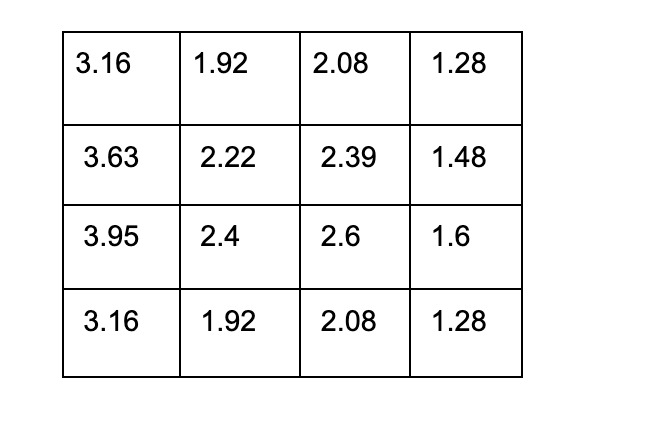
\includegraphics[width=11cm,height=4.8cm]{images/factorisation_result.jpeg}
\caption[Décomposition de la matrice]{Décomposition de la matrice}
\label{monlabel}
\end{center}
\end{figure}
\end{frame}

\begin{frame}{Neural Collaborative Filtering (NFC)}
\begin{figure}[h]
\begin{center}
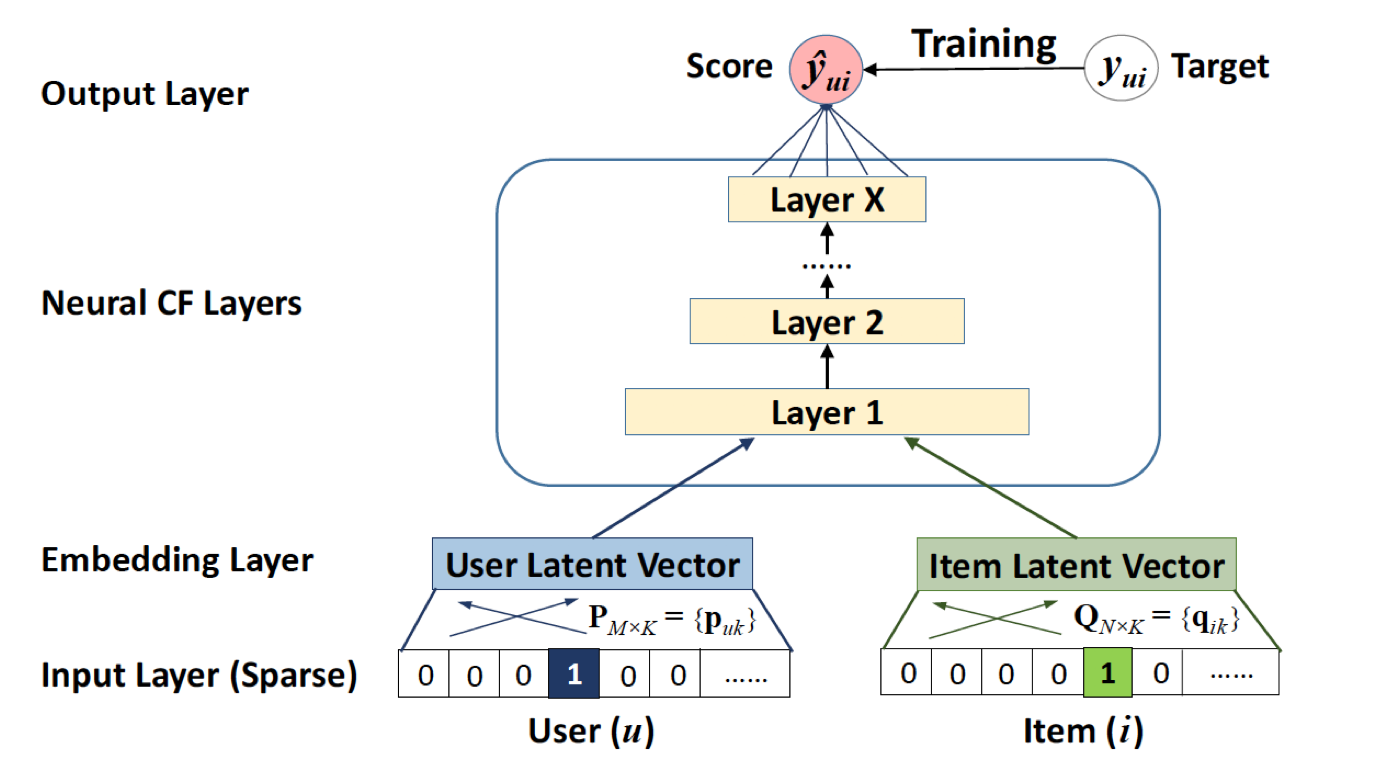
\includegraphics[width=11cm,height=4.3cm]{images/neural_cf.png}
\caption[\scriptsize{Neural Colaborative Filtering, https://towardsdatascience.com/neural-collaborative-filtering-96cef1009401}]{\scriptsize{Neural Colaborative Filtering, https://towardsdatascience.com/neural-collaborative-filtering-96cef1009401}}
\label{monlabel}
\end{center}
\end{figure}
\end{frame}

\begin{frame}{Généralisation du NFC}
\begin{figure}[h]
\begin{center}
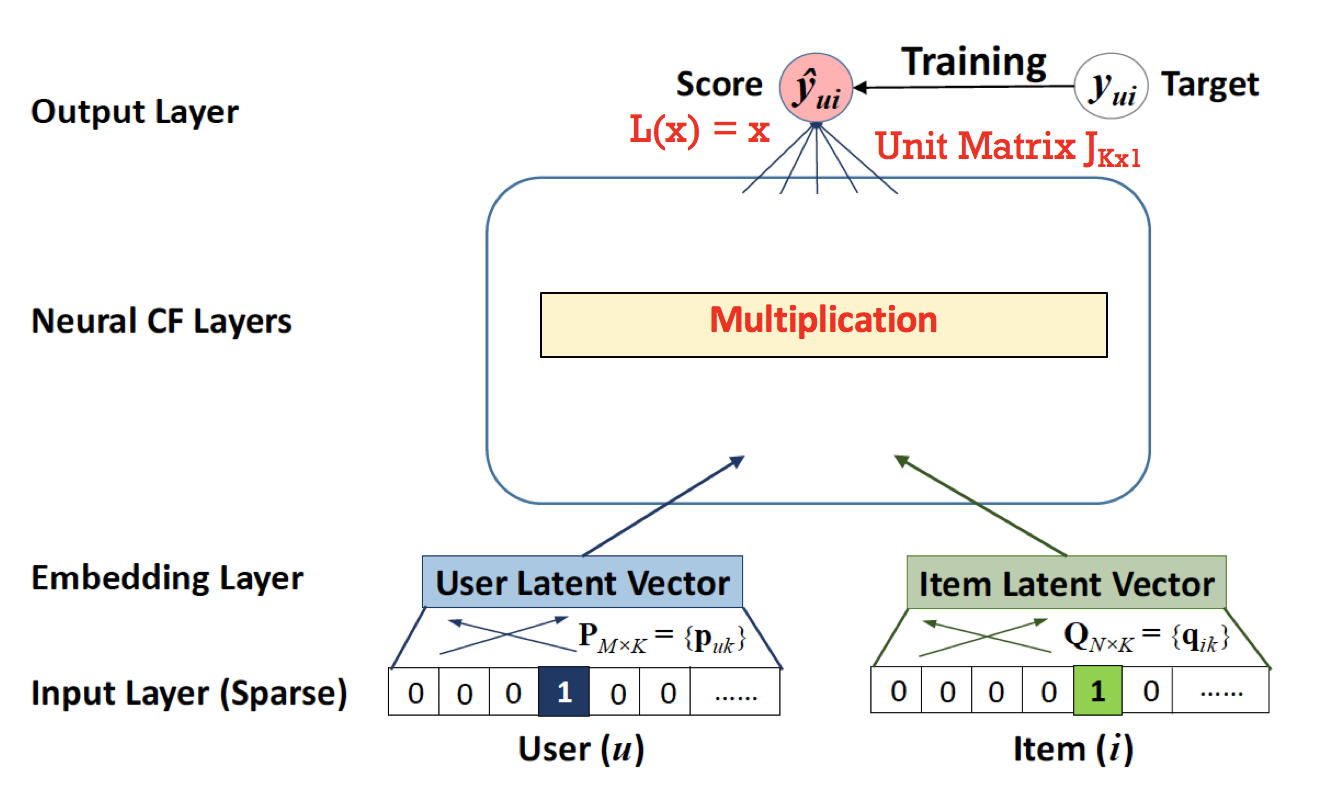
\includegraphics[width=11cm,height=4.3cm]{images/nfc_multiplication.png}
\caption[\scriptsize{Généralisation du NFC, https://towardsdatascience.com/neural-collaborative-filtering-96cef1009401}]{\scriptsize{Généralisation du NFC, https://towardsdatascience.com/neural-collaborative-filtering-96cef1009401}}
\label{monlabel}
\end{center}
\end{figure}
\end{frame}

\begin{frame}{Conditions de généralisation}
\begin{itemize}
  \item initialiser le poids de la couche de sortie à une matrice J dont toutes les valeurs sont égales à 1.
  \item Considérer une fonction d'activation L linéaire: 
  \end{itemize}
  $$L(x) = x$$
\end{frame}

\begin{frame}{Généralisation du NFC}
\begin{figure}[h]
\begin{center}
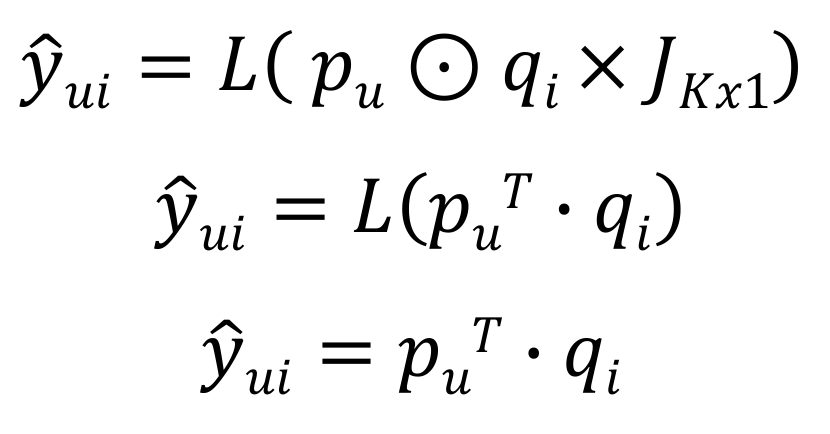
\includegraphics[width=7cm,height=3.5cm]{images/nfc_proof.png}
\caption[Généralisation du NFC]{Généralisation du NFC}
\label{monlabel}
\end{center}
\end{figure}
\end{frame}

\subsection{Combinaison des méthodes}
\begin{frame}{Combinaison des méthodes}
\begin{itemize}
  \item Combinaison du Collaborative Filtering au Content Based.
  \end{itemize}
\end{frame}

\subsection{Combinaison des méthodes}
\begin{frame}{Combinaison des méthodes}
\begin{itemize}
  \item Combinaison du Collaborative Filtering au Content Based.
  \end{itemize}
\end{frame}

\subsection{LSTM: Long Short Term Memory}
\begin{frame}{LSTM}
LSTM: Long Short Term Memory
\begin{itemize}
  	\item Famille de Réseau de Neurone Récurrent:
  		\begin{figure}[h]
\begin{center}
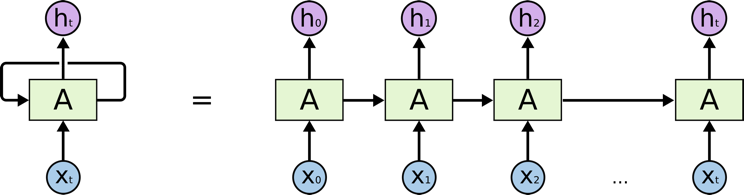
\includegraphics[width=8cm,height=2.5cm]{images/rnn_steps.png}
\caption[\scriptsize{Etats du RNN: https://towardsdatascience.com/understanding-lstm-and-its-quick-implementation-in-keras-for-sentiment-analysis-af410fd85b47}]{\scriptsize{Etats du RNN: https://towardsdatascience.com/understanding-lstm-and-its-quick-implementation-in-keras-for-sentiment-analysis-af410fd85b47}}
\label{monlabel}
\end{center}
\end{figure}
\end{itemize}
\end{frame}

\begin{frame}{LSTM}
\begin{itemize}
	\item Cas particulier du LSTM:\\
		  		\begin{figure}[h]
\begin{center}
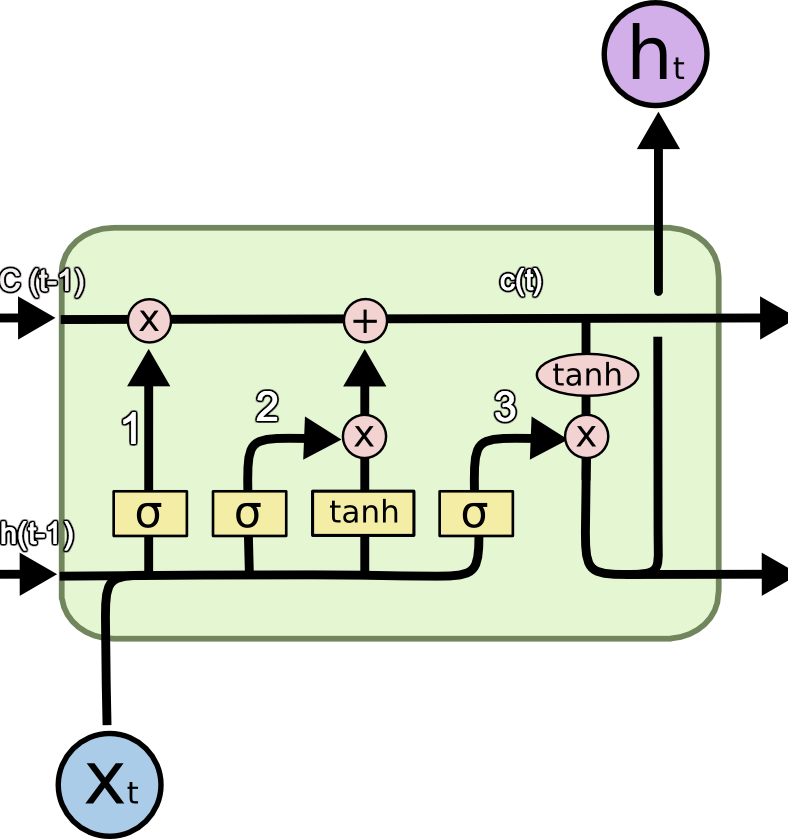
\includegraphics[width=6cm,height=4.5cm]{images/lstm_layer.png}
\caption[\scriptsize{Couche du LSTM: https://towardsdatascience.com/understanding-lstm-and-its-quick-implementation-in-keras-for-sentiment-analysis-af410fd85b47}]{\scriptsize{Couche du LSTM: https://towardsdatascience.com/understanding-lstm-and-its-quick-implementation-in-keras-for-sentiment-analysis-af410fd85b47}}
\label{monlabel}
\end{center}
\end{figure}

\end{itemize}
\end{frame}

\begin{frame}{LSTM}
\begin{itemize}
	\item Les différentes portes du LSTM:\\

	\begin{itemize}
  		\item Input Gate (Couche de Sigmoide $\sigma$):\\
Contrôle de quel vecteur entre en mémoire $c(t)$
\item Forget Gate (Couche de Sigmoide $\sigma$):\\
Contrôle de quel information supprimer de la mémoire $c(t)$
\item Candidate Gate (Couche de Sigmoide $tan(h)$):\\
Détermine quelle information écrire dans la mémoire $c(t)$.
	\item Output Gate (Couche de Sigmoide $\sigma$):\\
Détermine quelle information sort en sortie de la l’état caché. 
	\end{itemize}
\end{itemize}
\end{frame}

\section{Système réalisé}
\subsection{Analyse de données}
\begin{frame}{Aperçu du jeu de donnée}
\begin{figure}[h]
\begin{center}
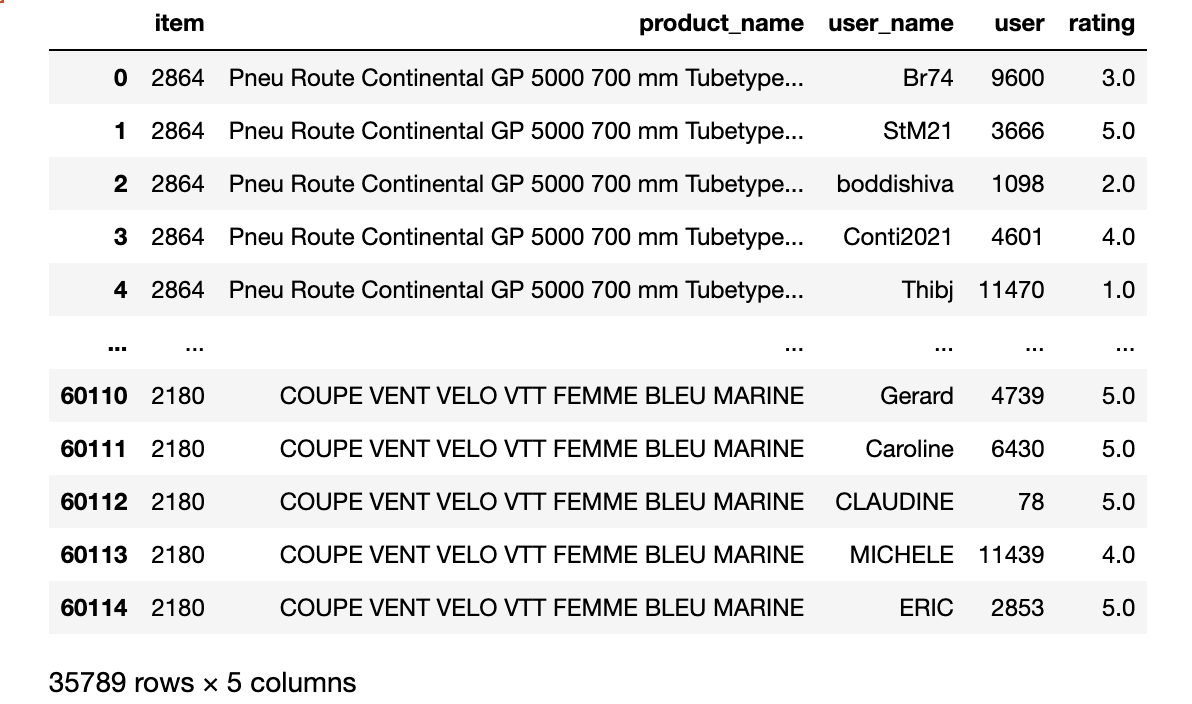
\includegraphics[width=10cm,height=6cm]{images/model_dataset.png}
\caption[Informations sur le produit le client et son vote]{Informations sur le produit le client et son vote}
\label{monlabel}
\end{center}
\end{figure}
\end{frame}

\begin{frame}{Statistiques sur la dataset:}
\begin{figure}[h]
\begin{center}
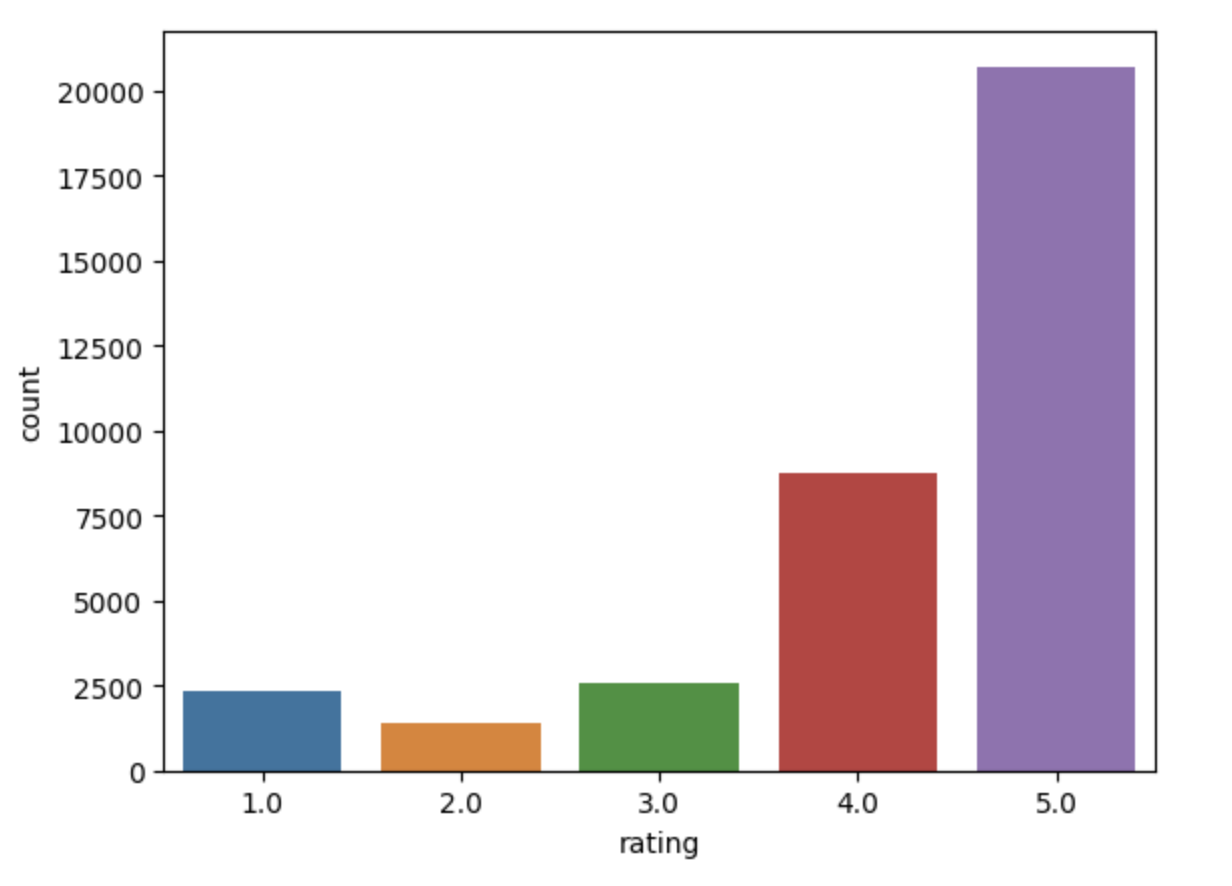
\includegraphics[width=8cm,height=5cm]{images/user_proportion.png}
\caption[Nombre de produits votés en fonction du score]{Nombre de produits votés en fonction du score}
\label{monlabel}
\end{center}
\end{figure}
\end{frame}

\begin{frame}{Statistiques sur la dataset:}
\begin{figure}[h]
\begin{center}
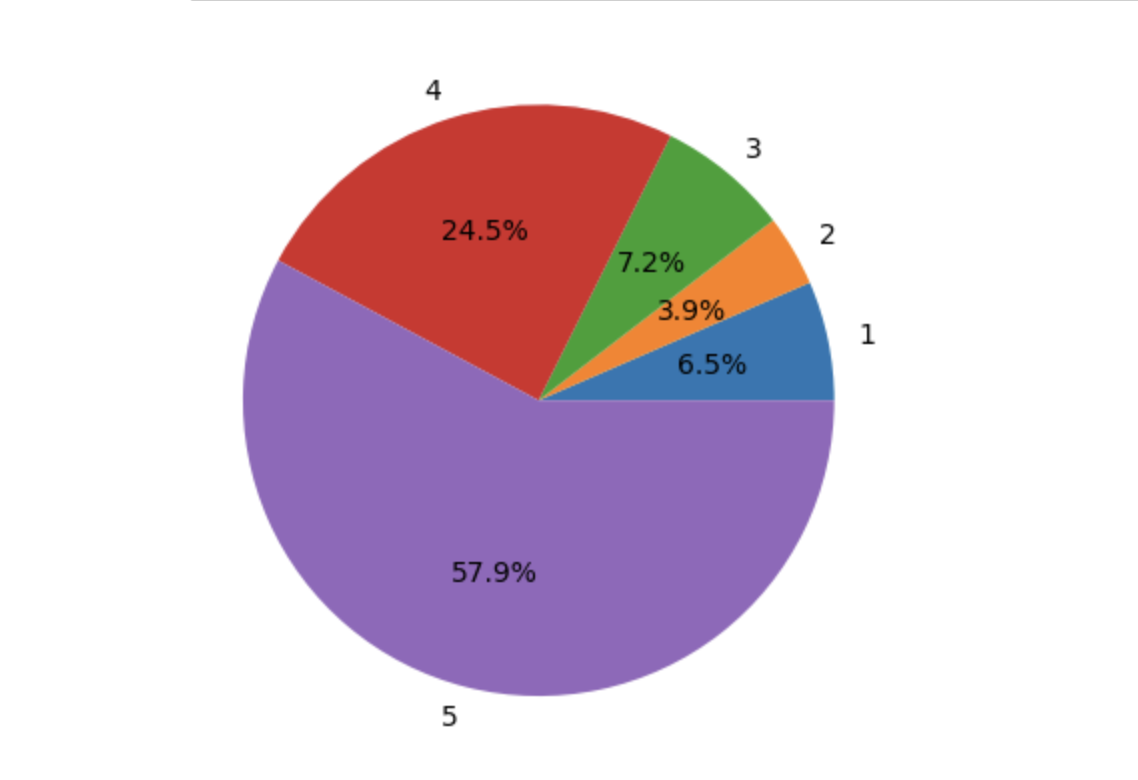
\includegraphics[width=8cm,height=5cm]{images/pie_user_vote.png}
\caption[Proportion du nombre de produits votés en fonction du score]{Proportion du nombre de produits votés en fonction du score}
\label{monlabel}
\end{center}
\end{figure}
\end{frame}

\begin{frame}{Différents modèles testés}
	\begin{itemize}
  		\item Matrice de Factorisation:
		\item Matrice de Factorisation et Réseau de Neurone:
		\item Matrice de Factorisation et Multilayer perceptron:
		\item LSTM: Long Short Term Memory:
	\end{itemize}
\end{frame}

\begin{frame}{Performances des modèles}
\begin{figure}[!htb]
\begin{center}
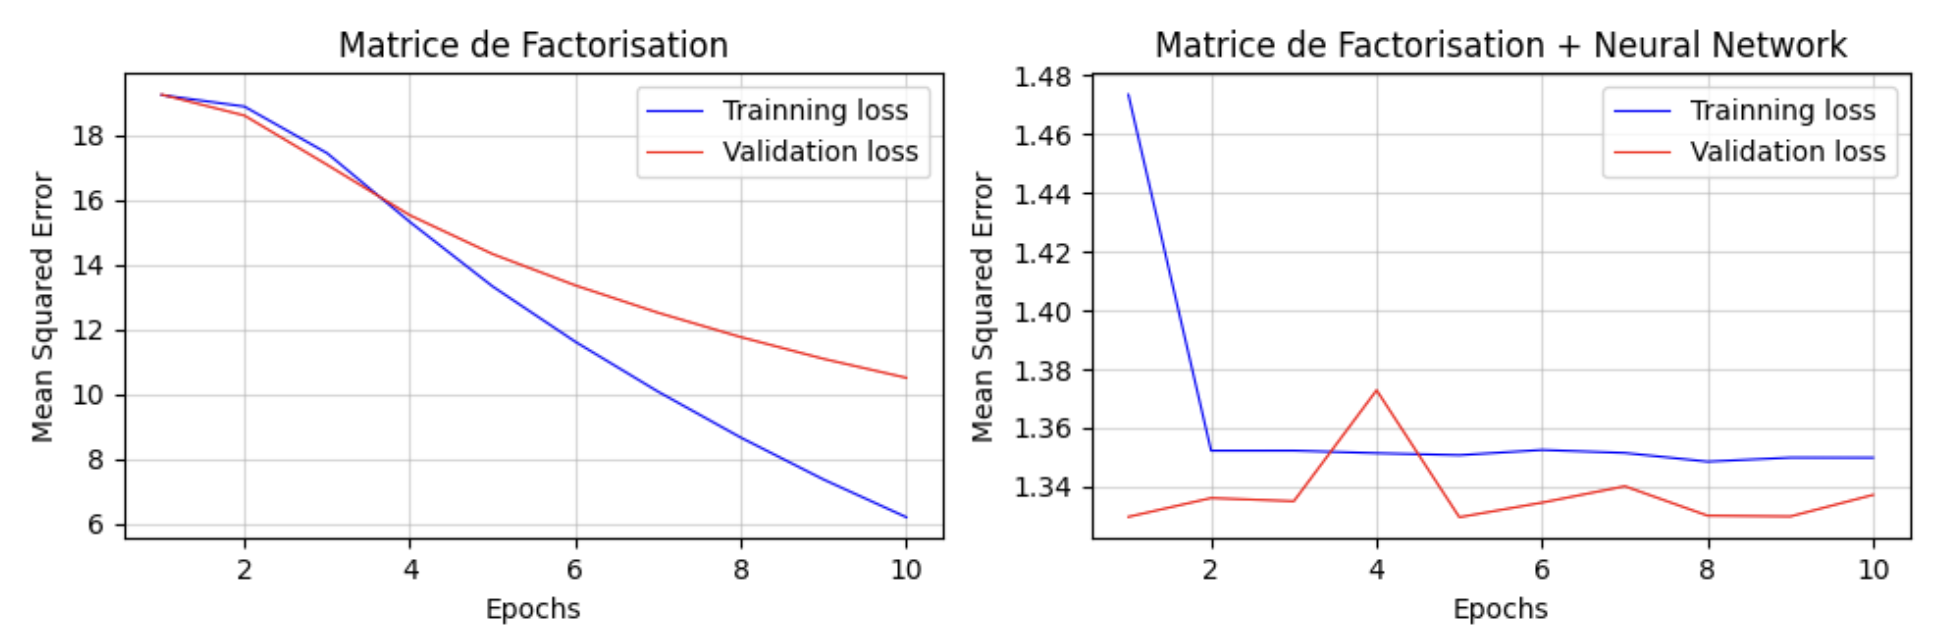
\includegraphics[width=11.5cm,height=4.9cm]{images/validation_mode_1.png}
\caption[Etude de la validation des modèles]{Etude de la validation des modèles}
\label{monlabel}
\end{center}
\end{figure}
\end{frame}

\begin{frame}{Performances des modèles}
\begin{figure}[!htb]
\begin{center}
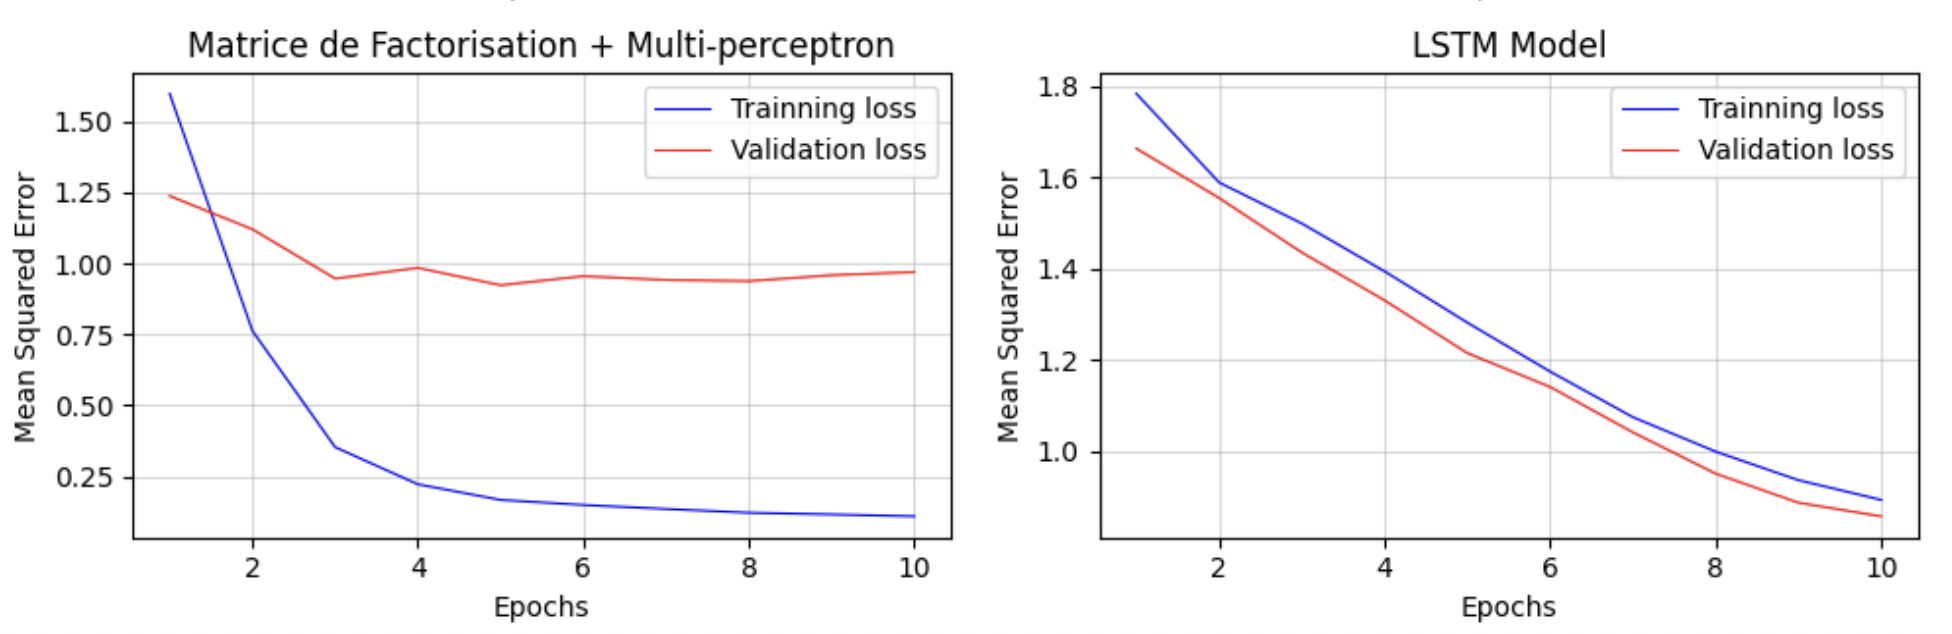
\includegraphics[width=11.5cm,height=4.9cm]{images/validation_mode_2.png}
\caption[Etude de la validation des modèles]{Etude de la validation des modèles}
\label{monlabel}
\end{center}
\end{figure}
\end{frame}

\begin{frame}{Performances des modèles}
\begin{figure}[!htb]
\begin{center}
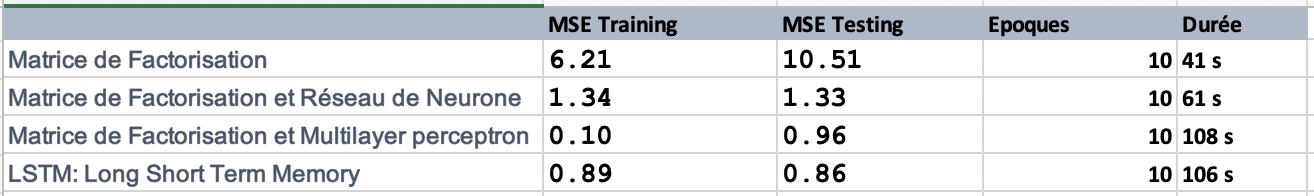
\includegraphics[width=11.5cm,height=2.5cm]{images/validation_statistics.png}
\caption[Statistiques de performances des modèles]{Statistiques de performances des modèles }
\label{monlabel}
\end{center}
\end{figure}
\end{frame}

\section{Conclusion}
\begin{frame}{Conclusion}
  \begin{itemize}
 \item La méthode de Deep Learning généralise au mieux la Matrice de Factorisation.
 \item Succès du modèle issu de la combinaison Matrice de Factorisation et Multilayer-Perceptron.
 \item Ajout de nouvelles données pour améliorer la performances des modèles.
 \item Combiner les votes aux avis dans la recommandation.
  
  \end{itemize}
  \end{frame}

% éléments hors section
\begin{frame}
\frametitle{Références}
\begin{thebibliography}{9}
\bibitem{texbook}
Sumit Sidana. Recommendation systems for online advertising. Computers and Society [cs.CY].
Université Grenoble Alpes, 2018. English. ffNNT : 2018GREAM061ff. fftel-02060436ff

\bibitem{texbook}
D Gunawan et al. The Implementation of Cosine Similarity to Calculate Text Relevance between Two Documents. 2018 J. Phys. : Conf. Ser. 978 012120



\end{thebibliography}
\end{frame}


\begin{frame}

\frametitle{Références}
\begin{thebibliography}{9}
\bibitem{lamport94}
Chakrabarti S, van den Berg M, Dom B 1999 Focused crawling : a new approach to topic-specific Web resource discovery Comput. Networks 31 11–16 pp 1623–1640

\end{thebibliography}
\end{frame}

\begin{frame}
  \begin{block}{}
  \centering
  Merci pour votre attention
  \end{block}
\end{frame}


\end{document}

